\chapter{Large Instances}
\label{chap:prelim}

\section{SAT-like Hamiltonian}
\begin{figure}[h]
	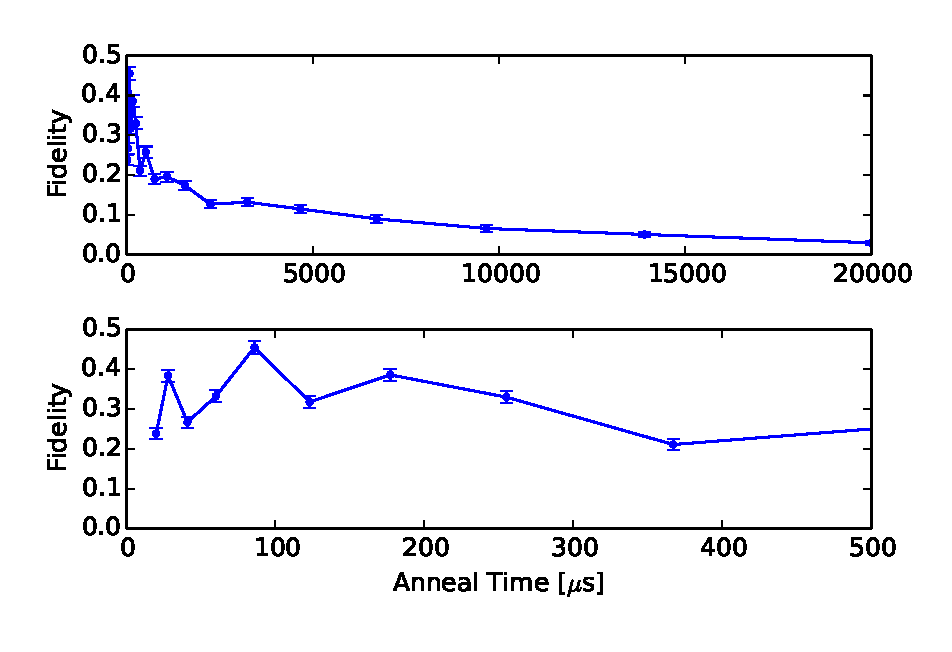
\includegraphics{img/6_018_2_fidelity.eps}
	\caption[Fidelity vs Time]{Plot of the fidelity as a function of annealing time for the Hamiltonian ``6\_018'' for both the full time range and the first 10 time points.  Both windows show the same data set.  Errors are estimated from $\sigma = \sqrt{np(1-p)}$.  Interesting features include the decrease in fidelity with longer anneal time and that the fidelity is very volatile over the short anneal time periods.}
	\label{fig:fidelity}
\end{figure}

Preliminary results were gathered on a sample quasi-random Hamiltonian called ``6\_018''.  This problem Hamiltonian was built up of clusters of clause sub-Hamiltonians in the same way as a SAT solver Hamiltonian would be, although ``6\_018'' does not encode a actual SAT problem.  This Hamiltonian was simple to generate and allowed us to verify our procedure for analyzing AQC results.
Data was collected in a series of evolutions at annealing times ranging from 20 $\mu$s to 20 ms.  Each evolution consists of choosing an anneal time and programming the problem Hamiltonian onto the hardware, then annealing 1000 times successively and reading out the final states.  We call each of these individual evaluations a \emph{read}, and a whole sequence of reads with the same programmed Hamiltonian a \emph{run}.  Any programming error (see \ref{sec:noise}) in the Hamiltonian should be the same between reads and differ between runs.

The state read out after each read is either the ground state, or some other higher energy (and incorrect) state.  The successes and failures thus follow a binomial distribution; there is some probability $p$ of getting the ground state, and probability $1-p$ of getting a different state.
Our best estimate of the fidelity from a single run is thus the fraction of successes, or $p = \frac{gs}{n}$ for $gs$ reads of the ground state and $n$ total reads.  We can also estimate the error in our estimate of the fidelity, because the variance of a binomial distribution is $\sigma^2 = np(1-p)$.

Figure \ref{fig:fidelity} shows the results of an initial set of runs spanning annealing times from 20 $\mu$s to 20 ms.  
There are several features of this data that stand out.  

Figure \ref{fig:short_fidelity} shows the same data as in Figure \ref{fig:fidelity} as well as three more sweeps conducted in the same fashion, annealing out to 500 $\mu$s.  The large-short time oscillations are still seen, and of note is the fact that different runs of the same anneal time lie far outside their respective error margins.  This confirms our earlier suspicion that rather than the quantum annealing fidelity actually changing so rapidly with small changes in anneal time, there is some other uncontrolled factor which is changing from run to run.

\begin{figure}
	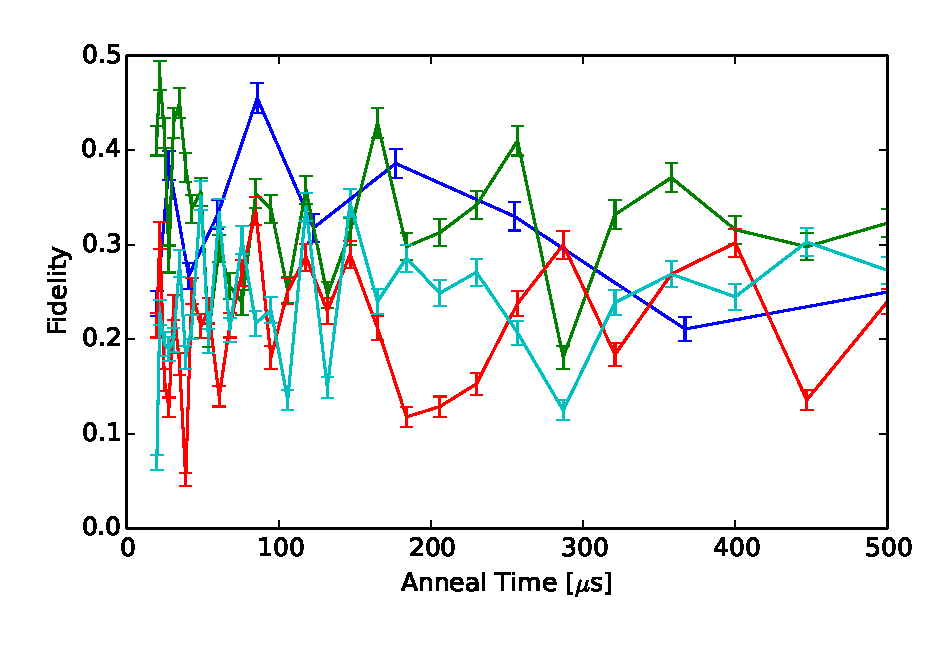
\includegraphics{img/6_018_comparison.eps}
	\caption[Short Time Fidelities]{The fidelity as a function of time for the Hamiltonian ``6\_018'' for several different machine runs.  Each data point consist of 1000 machine reads.  Notice the spread between machine runs is outside of the error bars.}
	\label{fig:short_fidelity}
\end{figure}





Unfortunately there is not much we can do with such low fidelities, so the rest of the results will focus on simpler Hamiltonians such as ones which occupy single K44s.  This means we cannot benchmark the \machine machine to any degree as was the initial plan since actual 3-SAT problems, even those as small as 6 problem variables, are too difficult for the machine to solve reliably.

Having carried out these preliminary results, we have established a framework for evaluating the \machine machine: ascertain the cause of the large uncertainty in the short-time evolution results, using simpler Hamiltonians; measure the effect that number of spins has in a more fine grained manner; and check the intra-run results to see how much of an effect read noise has.


The main Hamiltonian for the rest of the results will be ``k44\_and'', a single qubyte Hamiltonian similar to ``k44'' but featuring only a single non-degenerate ground state.


\begin{figure}
	\scalebox{0.4}{
		\includegraphics[bb= 0 0 1341 868]{img/4th_run_avg_low.png}
	}
	\caption[Running Fidelity Average]{Running average of the fidelity of the Hamiltonian ``6\_018'' for several short-time anneals, showing the change in fidelity with increasing read number.  The number of reads averaged over increases from zero to one thousand.  The rightmost edge of each data set shows the final fidelity estimate for that anneal time.  }
	\label{fig:running_avg}

\end{figure}
\section{Read noise}
First we examine the question of whether there is significant drift in the fidelity within a single run.  That is, does the probability of getting the ground state on any given read depend on the read number (the first read, second read etc.).  This question was examined on the Hamiltonian ``6\_018'' because the data collected on that particular Hamiltonian always consisted of at least 1000 reads per run.
Figure \ref{fig:running_avg} shows the running average of some short-time anneals from a single sweep of ``6\_018''.  If there is not significant read noise, we expect that the running average should flatten out and converge on the ``true'' fidelity after the appropriate number of reads.  For example, for a standard deviation $\sigma = \sqrt{np(1-p)}$ we expect that the running average should be within 5\% of the true fidelity after $\sim$ 200 reads.  Most of the anneal times appear to be reasonably flat past $\sim$ 500 reads, so the running averages appear to indicate to us that there isn't significant read noise (or at least, not nearly enough to be responsible for the short-time oscillations we saw in Chapter \ref{chap:prelim}).

The running average is a somewhat flawed quantity however, since it privileges earlier reads over later ones (since each read contributes like $1/N$ for $N$ reads already counted).  To remedy this we can also look at a rolling average of the fidelity as the reads come in.  Figure \ref{fig:rolling_avg} shows a rolling average of the fidelity for the same data as Figure \ref{fig:running_avg}.  Each point is the ground state fraction of the 100 reads around the labelled point; e.g. the value at point 500 is the number of ground states found from reads 450 to 550 over 100.  The rolling average has an advantage over the running average in that it does not prefer any part of the data set, but it can be harder to make out trends than in the running average.  It can be seen in the rolling average data that there does not appear to be a trend toward the fidelity being higher or lower in different segments of the run; e.g. the 22 $\mu$s run has highest fidelity in the nieghbourhood of read 600, while the 25 $\mu$s run has a minimum in the same location.

The combined results of the running and rolling averages would seem to indicate that intra-run errors, or errors occurring in the process of administering different reads, are not a significant contributor to the final observed fidelity for any given problem.

\begin{figure}
	\scalebox{0.35}{
		\includegraphics[bb=0 0 1582 917]{img/4th_run_roll_avg_low_100.png}
	}
	\caption[Rolling Fidelity Average]{Rolling average of the estimated fidelity for data collected from Hamiltonian ``6\_018'' at the seven shortest anneal times.  Each point is the average fidelity over a one hundred point window, e.g. the value at point 500 is the total number of times the ground state was measured between reads 450 and 550 divided by one hundred.}
	\label{fig:rolling_avg}
\end{figure}
